% type, article (not too long of a pdf) useful for assignments
\documentclass{article}

% List of packages needed for LaTeX document
\usepackage{graphicx}
\usepackage{import}
\usepackage{geometry}
\usepackage{hyperref}

% Tell the graphics package where to look for images
\graphicspath{ {images/} }
% Change margin, lower inches more text on screen
\geometry{margin=1.5in}
% used for creating links to click on
\hypersetup{
	colorlinks=true,
	linkcolor=black, %change colour simply e.g. linkcolor=blue
	filecolor=magenta,
	urlcolor=cyan,
}
% title information will be shown when \maketitle is run
\title{
	{CSU22013/CSU33013: Group 10}\\
	{Requirements Document}\\
	{Blockchain Publishing System}\\
	{\large Propylon}
}
% authors of will be shown when \maketitle is run
\author{
	{By Anastasiya Bogoslovskaya,}\\
	{Steven Cataluna,} \\
	{Charles Christiansson,} \\
    {Mohamed Difallah,} \\
	{Alice Doherty,} \\
	{Conor Doherty,} \\
	{Alexander Sepelenco}
}
\date{} % empty date{} means the pdf will have no date

\begin{document} % Acts like a main() function in programming (everything is drawn here)
\begin{figure}[h]
\centering % centre is you want
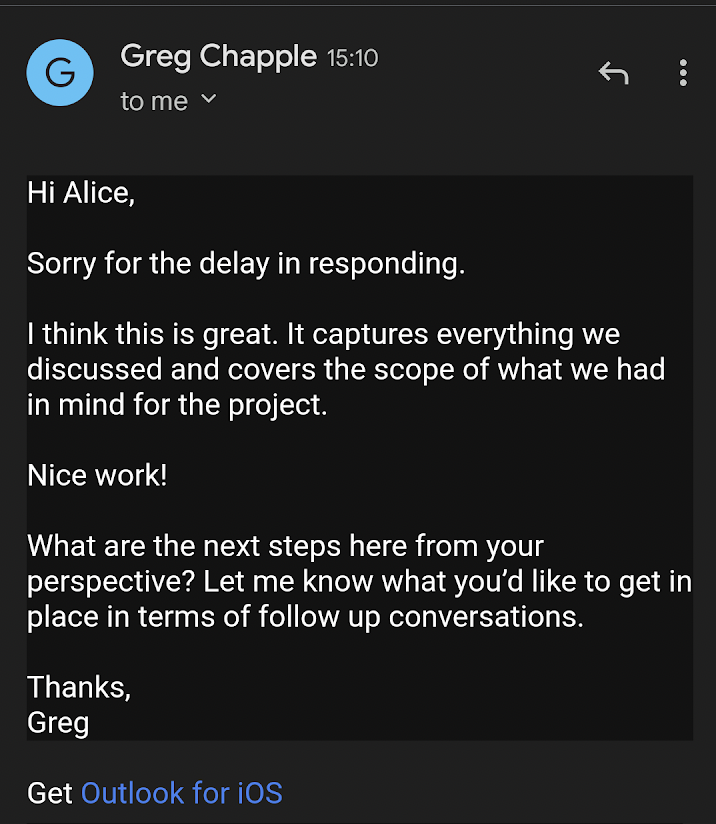
\includegraphics[scale=0.5]{gc-confirmation} % To learn more go to: https://www.overleaf.com/learn/latex/Inserting_Images 
\caption{Confirmation from Greg Chapple}
\label{fig: gc-confirmation} % Can be used with function \ref{fig: passion-fruit-flower} to reference to image
\end{figure}

\maketitle % This will add title, and authors to the pdf 
\tableofcontents % Automatically figure out the contents looking at \section \subsection \subsubsection 

% specify location to import .tex files from so that we can keep things modular and not in one big file
\import{./Sections/}{Introduction} 
\import{./Sections/}{Current-System}
\import{./Sections/}{Proposed-System}

\end{document} % End of main function
